Lex est un analyseur lexical, c'est à dire que celui-ci permet de transformer une suite de symboles en terminaux (un terminal peut être une lettre, un chiffre, un signe '*' ...). Après cette transformation faite, le main est repassé à l'analyseur syntaxique. Par conséquent, le but de cette analyseur lexical est de "prendre" des symboles, de les transformer en respectant ces règles qui lui sont propres et les donner à l'analyseur syntaxique. Chaque règles sont représenté sous la forme d'une expression régulière et d'actions. Dans ce cas, si un "match" a lieu entre l'expression saisie et l'expression régulière définit alors les actions qui lui sont associée sont exécutées.
La compilation d'un programme en Lex génère un programme C/C++ et ce programme définit la fonction yylex(void) qui permet de représenter l'analyseur lexical.

Il faut savoir qu'un programme Lex possède 4 parties :
\begin{verbatim}
    %{ (Optionnel)
    Partie 1 : déclarations pour le compilateur C (Optionnel)
    %} (Optionnel)
    Partie 2 : définitions régulières (Optionnel)
    %%
    Partie 3 : règles (Optionnel)
    %% (Optionnel)
    Partie 4 : fonctions C supplémentaires (Optionnel)
\end{verbatim}

\subsection{Partie 1}
Cette partie permet de spécifier les fichiers à inclure ("\#include ..."). Ces lignes seront tout simplement copié au début du fichier généré.

\subsection{Partie 2}
Dans cette partie se trouve les définitions régulières qui permet donc de définir des notions non terminales. La forme de ces définition régulières doivent être :
\begin{verbatim}
NON-TERMINALE   EXPRESSION_REGULIERE
\end{verbatim}

Par exemple :

\begin{verbatim}
character [a-zA-Z]
digit [0-9]
word ({charater}|{digit})+
\end{verbatim}

\subsection{Partie 3}
C'est dans cette troisième partie que se trouve les différentes règles. Une action est un morceau de code C, qui sera recopie tel quel, au bon endroit, dans la fonction yylex. Ces différentes reglès devront être sous la forme : 

\begin{verbatim}
EXPRESSION_REGULIERE {ACTIONS}
\end{verbatim}

Par exemple :

\begin{verbatim}
yacc    printf("(1)%s",yytext);
word    {printf("word : "); printf("%s", yytext);} 
\end{verbatim}

NB: Il est possible d'effectuer plusieurs actions pour une même expression régulière (elles doit se trouver entre "\{...\}"). Si une expression régulière ne possède pas d'action alors Lex recopiera les caractères tels quels sur la sortie standard.

\subsection{Partie 4}
Dans cette dernière partie se trouve du code C qui sera tout simplement copié à la fin du fichier généré. Si celle-ci est vide alors le compilateur prendra le main dit par défaut qui est :
\begin{verbatim}
main() {
  yylex();
}
\end{verbatim}

\subsection{Exemple pour compiler un fichier Lex} 
Vous trouverez dans la racine du dossier de ce rapport un fichiers Lex qui se nomme "essai\_lex.lex". Voici les différentes commandes à effectuer :

\begin{verbatim}
$ lex essai_lex.lex
$ mv lex.yy.c essai_lex.lex.c
$ gcc essai_lex.lex.c -ll
$ ./a.out < textlex
\end{verbatim}


Le résultat de ce code est le suivant :

\begin{figure}[h]
    \centerline{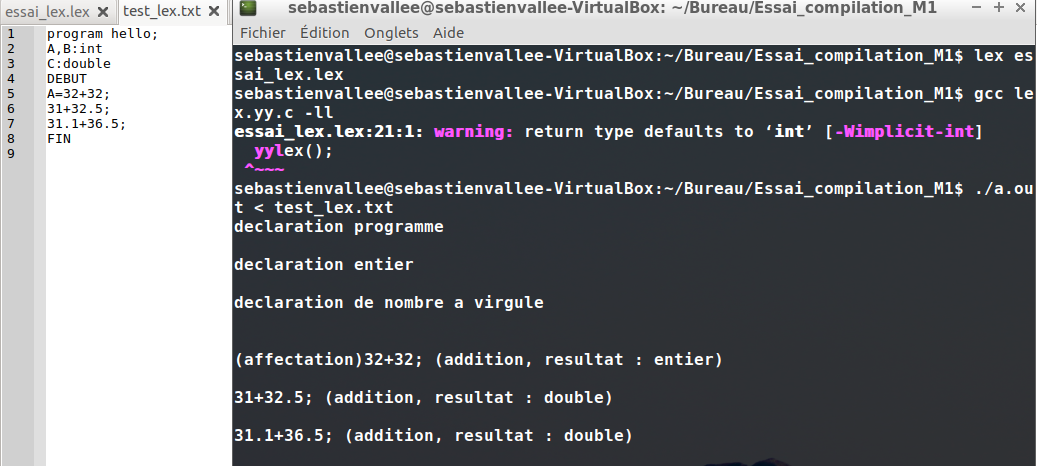
\includegraphics[scale=0.6]{data/lex}}
    \caption{Résultat du code lex}
    \label{fig:lex}
\end{figure}

Sur la figure \href{fig:lex}{1},  on peut voir que le but du programme est de remplacer les lignes du programme du fichier en entrée, par une description des expression qu'il trouve. Par exemple, on peut lire sur la sortie standard que la deuxième ligne du programme est une déclaration d'entier ; ou que l'addition 32+32 est précédé d'une affectation à une variable, tandis que les deux additions suivante non.
Lorsque qu'un mot n'est pas reconnu par Lex, il est par défaut envoyé sur la sortie standard, ce qui n'est pas le cas pour ce mot (le fichier en entrée).

Alors bien que Lex peut offrir des outils puissant, l'analyse de fichiers peut s'avérer assez difficile. On ne peut par exemple, pas savoir si les additions sont bien entre les balises "DEBUT" et "FIN" (sauf en écrivant un code c inutilement compliqué). Nous verrons plus tard qu'un autre outil est plus puissant dans ces cas là.